\documentclass{standalone}

\usepackage{tikz}
\usepackage{circuitikz}

\tikzset{block/.style = {draw, fill=white, very thick, rectangle, minimum height=1cm, minimum width=2cm},
         lblock/.style={draw,fill=white,very thick, rectangle, minimum height=3cm, minimum width=1cm},
         sum/.style= {draw, fill=white, very thick, circle, node distance=0.5cm}}

         
\begin{document}
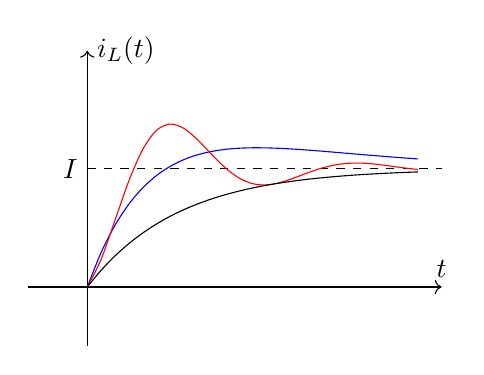
\begin{tikzpicture}[scale=1.5]
    \draw[->](-0.5,0)--(3,0)node[above]{$t$};
    \draw[->](0,-0.5)--(0,2)node[right]{$i_L(t)$};
    \draw[dashed](0,1)node[left]{$I$}--(3,1);

    \draw[blue]plot[smooth, domain=0:2.8](\x,{1+1.5*\x*e^(-1.3*\x)-e^(-1.3*\x)});        
    \draw[red]plot[smooth, domain=0:2.8](\x,{1-e^(-1.3*\x)*cos(4*\x r)});
    \draw[black]plot[smooth, domain=0:2.8](\x,{1-e^(-1.3*\x)});
\end{tikzpicture}
\end{document}